% File: analyse.tex
% Date: Fri Aug 31 00:50:20 2012 +0800
% Author: Yuxin Wu <ppwwyyxxc@gmail.com>
\section{Results and Analysis}
各参数对程序运行时间的影响:

\begin{enumerate}
	\item iter:\\
		程序在判断一个点是否属于集合中时,对一点迭代iter次,iter越高,所得图像越精确,集合边界越清晰,所花时间也越长.
		同时,由于程序配色函数比较特殊,iter取值的改变可能使得集合周围显示一些美妙图案.
		
		迭代次数极少时,集合边界非常圆滑,随着迭代次数增加,边界向内收缩.如\figref{shrink}


		\begin{figure}[H]
			\centering
			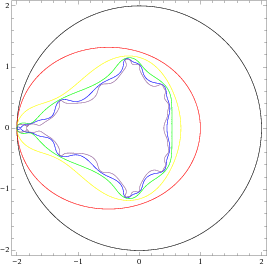
\includegraphics[scale=1]{res/shrink.png}
			\caption{\label{fig:shrink}}
		\end{figure}

\begin{lstlisting}
$ ./pthread -s 2000x2000 -i 1000
0.622379 seconds elapsed
$ ./pthread -s 2000x2000 -i 5000
2.880889 seconds elapsed
$ ./pthread -s 2000x2000 -i 8000
4.572143 seconds elapsed
$
\end{lstlisting}
从以上速度测试可以看出,iter增加到$ k$倍时,耗时略小于$ k$倍.这是因为对区域中的许多点,经过少量迭代就已经越界.


\item size:\\
\begin{lstlisting}
$ ./pthread -s 1000x1000
0.157242 seconds elapsed
$ ./pthread -s 2000x2000
0.622366 seconds elapsed
$ ./pthread -s 3000x3000
1.396862 seconds elapsed
$ ./pthread -s 4000x4000
2.478775 seconds elapsed
\end{lstlisting}
从数据可以看出,耗时的变化大约与点的个数成正比,耗时略少于$ k$倍,猜想是多线程的启动耗时,openmp,MPI也有类似情况.于是增大数据规模:


\begin{lstlisting}
$ ./pthread -s 10000x10000 -i 300
5.636299 seconds elapsed
$ ./pthread -s 10000x20000 -i 300
11.265757 seconds elapsed
$ ./pthread -s 20000x20000 -i 300
22.500245 seconds elapsed
$ ./pthread -s 20000x40000 -i 300
46.199222 seconds elapsed
$ ./pthread -s 30000x40000 -i 300
71.325897 seconds elapsed
\end{lstlisting}

数据规模变大后,线程启动耗时的影响渐渐可以忽略不计,此时可以看出,数据规模变为$ k$倍时,程序耗时略多于$ k$倍,这应当是线程间锁定/进程间通信耗时的结果.

\item domain:\\
	由于区域各点所执行的迭代次数不同,改变区域可能大幅改变程序效率.

\begin{lstlisting}
$ ./pthread -d -5,-5,2,2
0.008872 seconds elapsed
$ ./pthread -d -0.2,-0.2,0.1,0.1   
0.974035 seconds elapsed
\end{lstlisting}

\item nproc:\\
	使用pthread加速时,通过命令行参数改变nproc:
\begin{lstlisting}
$ ./pthread -n 2 -s 5000x5000
7.524309 seconds elapsed
$ ./pthread -n 4 -s 5000x5000                                                                                                                                                                                                                  
3.761441 seconds elapsed
$ ./pthread -n 8 -s 5000x5000
1.882019 seconds elapsed
$ ./pthread -n 16 -s 5000x5000
1.894062 seconds elapsed
$ ./pthread -n 32 -s 5000x5000
1.935740 seconds elapsed
\end{lstlisting}
	使用MPI加速时,利用mpirun改变nproc:
\begin{lstlisting}
$ mpirun -n 2 ./mpi -s 5000x5000
15.010539 seconds elapsed
$ mpirun -n 4 ./mpi -s 5000x5000
5.037870 seconds elapsed
$ mpirun -n 6 ./mpi -s 5000x5000
3.273679 seconds elapsed
$ mpirun -n 8 ./mpi -s 5000x5000
2.186701 seconds elapsed
$ mpirun -n 9 ./mpi -s 5000x5000
2.895381 seconds elapsed
$ mpirun -n 16 ./mpi -s 5000x5000
3.586846 seconds elapsed
\end{lstlisting}

\begin{lstlisting}
$ ./omp -s 5000x5000
1.887277 seconds elapsed
\end{lstlisting}


\begin{figure}[H]
\centering
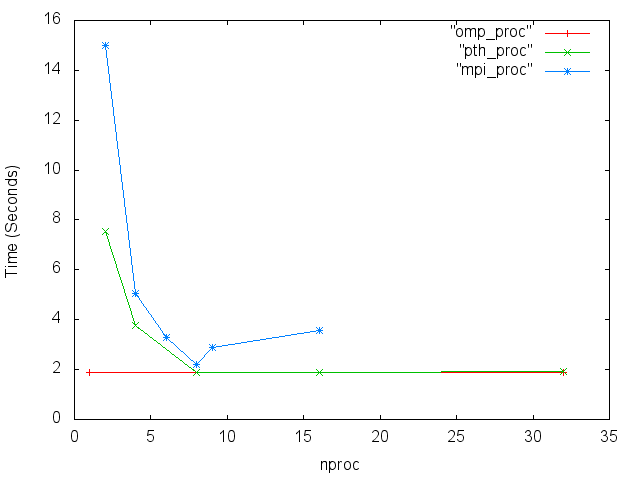
\includegraphics[scale=0.5]{res/chart.png}
\end{figure}

由以上数据(由清华大学FIT楼集群计算机生成)可以看出,对于pthread, 线程数等于处理器个数时最佳.对于MPI,由于此程序有一进程只负责管理任务,因此效率与进程数关系可能略有不同,无法与pthread进行直接比较.但从数据来看仍是8个进程时效率最高.
而且由于MPI的进程通信及初始化更为复杂,因此进程数更高时效率会明显下降.
OpenMP由于设置成自动分配,无法改变线程数,但其效率很高.

对于更大规模的数据,只能使用MPI进行多节点测试,测试数据如下.

\begin{table}[h]
	\centering
	\begin{tabular}{c|c}
		\hline
	nproc & time \\\hline
	24 & 373.262603 \\
	36 &281.326281 \\
	48 &203.073978\\
	60 &169.850154\\
	72 &157.953276 \\\hline
\end{tabular}
\end{table}

\begin{figure}[H]
	\centering
	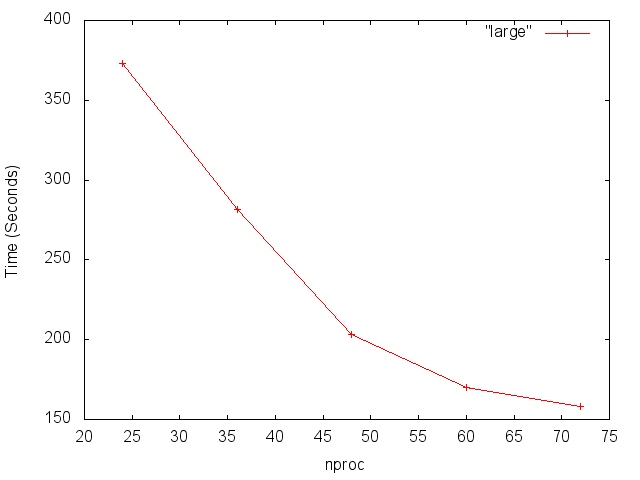
\includegraphics[scale=0.6]{res/large.png}
\end{figure}
测试参数: -s 30000x30000 -i 20000

\end{enumerate}
